\documentclass[a4paper,12pt]{article}
\usepackage[T2A]{fontenc}
\usepackage[utf8]{inputenc}
\usepackage[top=2cm, bottom=2cm, right=2cm, left=2cm]{geometry}
\usepackage[russian]{babel}
\usepackage{pscyr}
\usepackage{indentfirst}
\usepackage{graphicx}
\usepackage{epstopdf}
\usepackage{amstext}
\usepackage{amssymb}
\usepackage{amsmath}
\usepackage{cmap}
\usepackage{enumitem}
\usepackage{multirow}
\pdfminorversion=6
%\input{environment}
%\linespread{1.3}
\tolerance=1000 
\hfuzz=0pt
\parindent=1.27cm
\usepackage{subcaption}
\captionsetup[table]{name = Таблица, labelsep = endash, justification=raggedright, singlelinecheck=false}
\captionsetup[figure]{name = Рисунок, labelsep = endash}
%\sloppy
\RequirePackage{caption}
\DeclareCaptionLabelSeparator{defffis}{ -- }
\captionsetup{justification=centering,labelsep=defffis}
\usepackage{array}
\usepackage{subcaption}
\usepackage{pgfplots}
\usetikzlibrary{pgfplots.polar}
\pgfplotsset{compat=1.13}
\pgfplotsset{grid = major, grid style = {dashed}}
\usepackage{tabu}
\usepackage{threeparttable}
\usepackage{pgfplotstable}
\renewcommand{\arraystretch}{1.5}
% recommended:
\usepackage{booktabs}
\usepackage{colortbl}
\graphicspath{{images/}}

\begin{document}
	\newcommand\tline[2]{$\underset{\text{#1}}{\text{\underline{\hspace{#2}}}}$}
	\begin{titlepage}
		\centering
		{\fontsize{12pt}{5cm}\selectfont \bfseries Министерство образования и науки Российской Федерации} \\ \vspace{0.5cm}
		{\fontsize{7pt}{5cm}\selectfont ФЕДЕРАЛЬНОЕ ГОСУДАРСТВЕННОЕ АВТОНОМНОЕ ОБРАЗОВАТЕЛЬНОЕ УЧРЕЖДЕНИЕ ВЫСШЕГО ПРОФЕССИОНАЛЬНОГО ОБРАЗОВАНИЯ} \\ 
		\vspace{1cm}
		{\fontsize{12pt}{5cm}\selectfont \bfseries САНКТ-ПЕТЕРБУРГСКИЙ УНИВЕРСИТЕТ ИНФОРМАЦИОННЫХ ТЕХНОЛОГИЙ, МЕХАНИКИ И ОПТИКИ} \\ \vspace{1.5cm}

		{\fontsize{14pt}{5cm}\selectfont Кафедра \hspace{1cm} \underline{Систем Управления и Информатики}  \hspace{1cm} Группа \underline{Р3340}} \\ 
		\vspace{2cm}

		{\fontsize{20pt}{5cm}\selectfont \bfseries Лабораторная работа №11} \\
		{\fontsize{20pt}{5cm}\selectfont \bfseries “Исследование математической модели пьезоэлектрического исполнительного устройства”} \\
		{\fontsize{14pt}{5cm}\selectfont Вариант - 5} \\
		\vspace{1.5cm}

		\flushleft

		{Выполнил \hspace{2cm} \tline{(фамилия, и.о.)}{9cm} (подпись)} \\
		\vspace{2cm}

		{Проверил \hspace{2cm} \tline{(фамилия, и.о.)}{9cm} (подпись)} \\
		\vspace{5cm}

		"\underline{\hspace{0.7cm}}"\hspace{0.2cm}\underline{\hspace{2cm}}\hspace{0.2cm}20\underline{\hspace{0.7cm}}г. \hspace{2cm} Санкт-Петербург, \hspace{2cm} 20\underline{\hspace{0.7cm}}г. \\ \vspace{1cm}

		Работа выполнена с оценкой \hspace{1cm} \underline{\hspace{8cm}} \\ 
		\vspace{1cm}
		Дата защиты "\underline{\hspace{0.7cm}}"\hspace{0.2cm}\underline{\hspace{2cm}}\hspace{0.2cm}20\underline{\hspace{0.7cm}}г.

	\end{titlepage}
	\paragraph{Цель работы.}  Изучение математических моделей и исследование характеристик исполнительного устройства, построенного на основе пьезоэлектрического двигателя микроперемещений. 
	\paragraph {Исходные данные:} Представлены в таблице \ref{t_1}
	\begin{table}[h]
		\centering
		\caption{Исходные данные}
		\renewcommand{\arraystretch}{2} 
		\renewcommand{\tabcolsep}{0.85cm}
		\begin{center}
			\begin{tabular}{|c|c|c|c|c|c|}
				\hline
				$Cp$, Н/м & $m$, кг & $K_0$, Н/В & $K_d$, Нс/м & $T_u$, мс & $F_{\text{в}}$ \\ \hline
				0.6 $\cdot 10^8$ & 0.5 & 8.2 & 900 & 0.05 & 50  \\ \hline
			\end{tabular}
		\end{center}
		\label{t_1}
	\end{table}
	
	\paragraph {} Рассчет необходимых параметров модели:\\
	
	\noindent
	$K_u=\displaystyle\frac{U_{Pm}}{U_m}=\frac{300}{10}=30$\\
	
	Коэффициенты передачи измерительных устройств:\\
	
	\noindent
	$
	K_V=28.6\\
	K_F=0.0067\\
	K_X=1.45\cdot 10^5\\	
	$
	\newpage
	\begin{center}
		\section{Получение передаточных функций двигателя и системы}
	\end{center}
\par
		Для составления передаточной функции двигателя будем рассматривать пьезоэлектрическое устройство как упругую механическую систему. Тогда математическая модель может быть получена на основе уравнения баланса сил в пьезодвигателе:
		\begin{gather}
		F_y = F_O + F_\text{Д} + F_d + F_B,
		\label{v_1}
		\end{gather}\\
		
		где $F_y = C_p\cdot x, F_O = K_O\cdot U_p, F_\text{Д} = -m\displaystyle{\frac{d^2x}{d t}}$. Подставив перечисленные равенства в уравнение (\ref{v_1}), получим:
		\begin{gather}
		m\cdot\ddot{x} + K_d\cdot\dot{x} + C_p\cdot x = K_o\cdot U_p + F_B
		\end{gather}\\
		
		Следовательно, передаточная функция пьезоэлектрического двигателя при нулевом внешнем возмущении будет следующей:
		\begin{gather} \label{v_2}
		W_\text{ПД}(s) = \displaystyle{\frac{K_O}{ms^2 + K_ds + C_p}}.
		\end{gather}
		
		Управление ПД осуществляется с ВУ, который описывается апериодическим звеном первого порядка:
		\begin{gather}
		W_\text{ВУ}(s) = \frac{K_u}{T_us + 1},
		\end{gather}\\
		
		Так как ВУ и ПД соединены последовательно, то передаточная функция системы:
		\begin{gather}
		\label{v_3}
		W(s)=\frac{K_u\cdot K_o}{(T_u s+1)(ms^2+K_d s+C_p)} 
		\end{gather}
	
	
	
	\newpage
	\begin{center}
	\section{Исследование системы без возмущения}
	\end{center}
	\paragraph {} Схема моделирования представлена на рисунке \ref{s_1}
	
	\begin{figure}[h]
		\renewcommand{\figurename}{Рисунок}
		\centering
		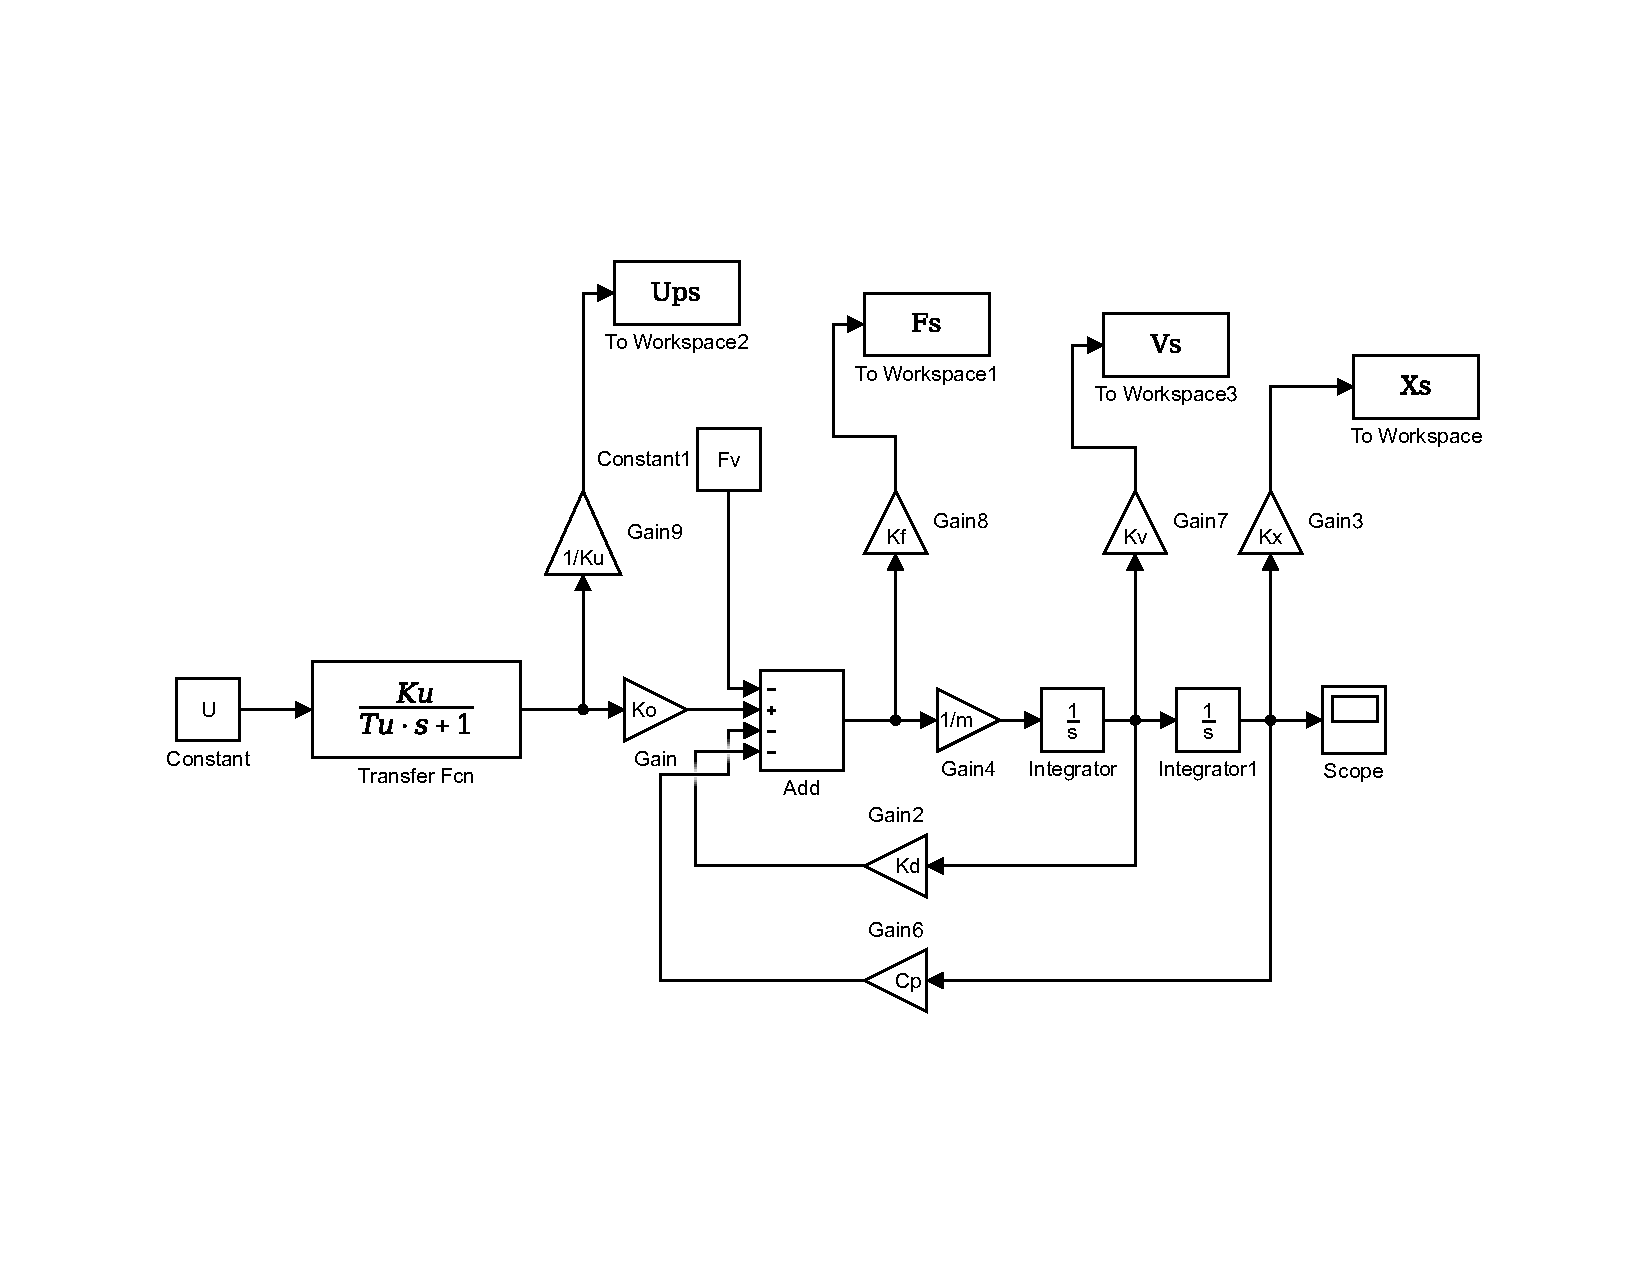
\includegraphics[width=6in]{Labb11.pdf}
		\caption{Схема моделирования}
		\label{s_1}
	\end{figure}
	%\newpage
	\paragraph {} Графики переходных процессов при $U=10$ и $F_{\text{в}}=0$ для каждого из исследуемых значений представлены на рисунке \ref{s_2}\\
	
	\begin{figure}[h!]
		\renewcommand{\figurename}{Рисунок}
		\begin{minipage}[h]{0.47\linewidth}
			\center{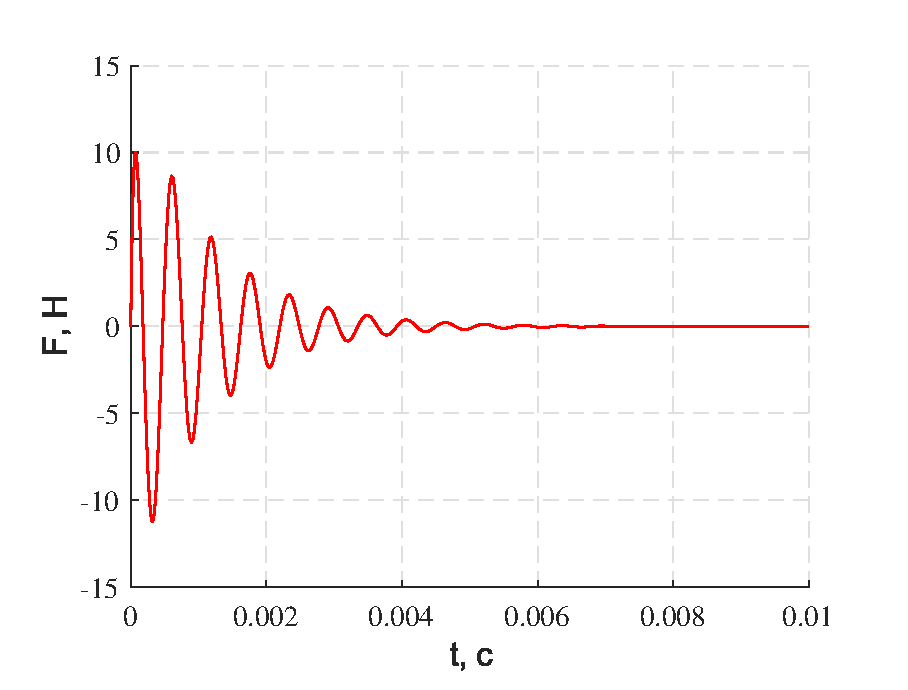
\includegraphics[width=1\linewidth]{phf1.eps}} a) \\
		\end{minipage}
		\hfill
		\begin{minipage}[h]{0.47\linewidth}
			\center{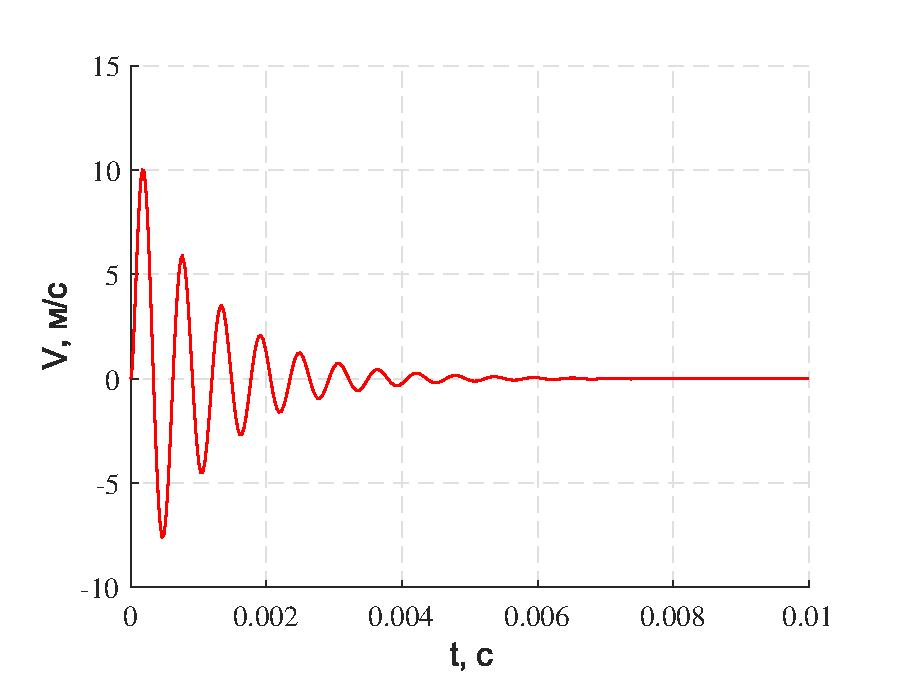
\includegraphics[width=1\linewidth]{phv1.eps}} \\b)
		\end{minipage}
		\vfill
		\begin{minipage}[h]{0.47\linewidth}
			\center{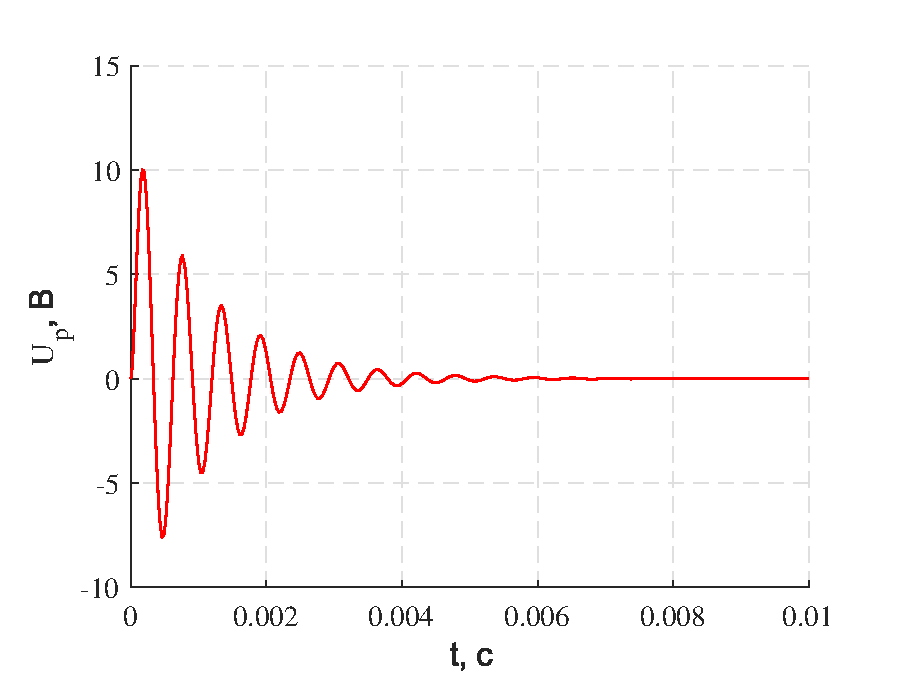
\includegraphics[width=1\linewidth]{phu1.eps}} c) \\
		\end{minipage}
		\hfill
		\begin{minipage}[h]{0.47\linewidth}
			\center{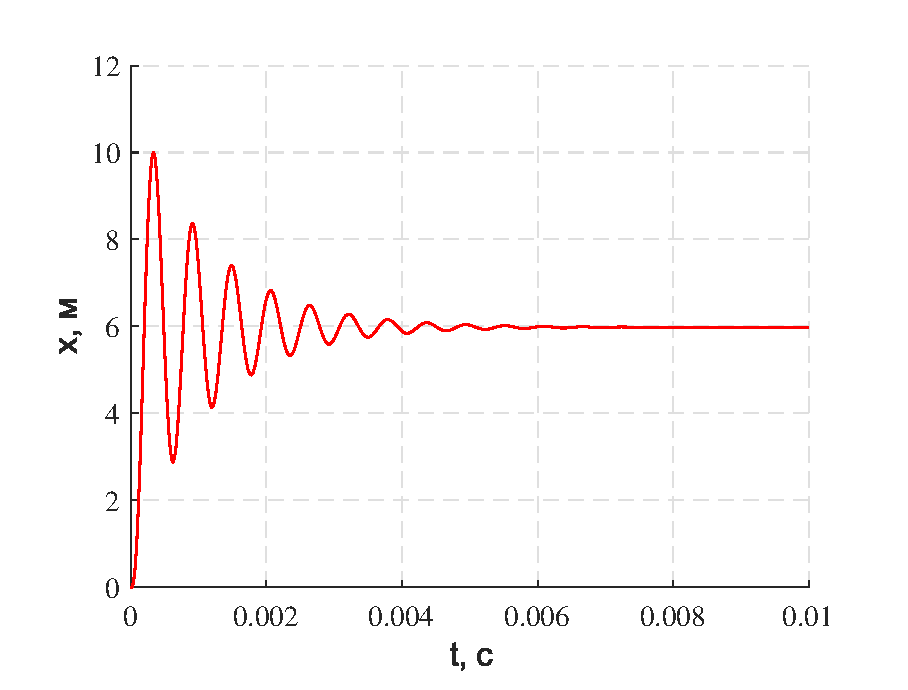
\includegraphics[width=1\linewidth]{phx1.eps}} d) \\
		\end{minipage}
		\caption{Переходные процессы: a) динамическое усилие, b)
			скорость, c) напряжение, d) перемещение}
		\label{s_2}
	\end{figure}

	\clearpage
	\begin{center}
	\section{Исследование влияния массы нагрузки $m$ на вид переходных процессов}
	\end{center}
		
		
			\paragraph {} Графики переходных процессов при различных $m$ для каждого из исследуемых значений представлены на рисунке \ref{s_3}\\
		
		\begin{figure}[h!]
			\renewcommand{\figurename}{Рисунок}
			\begin{minipage}[h]{0.47\linewidth}
				\center{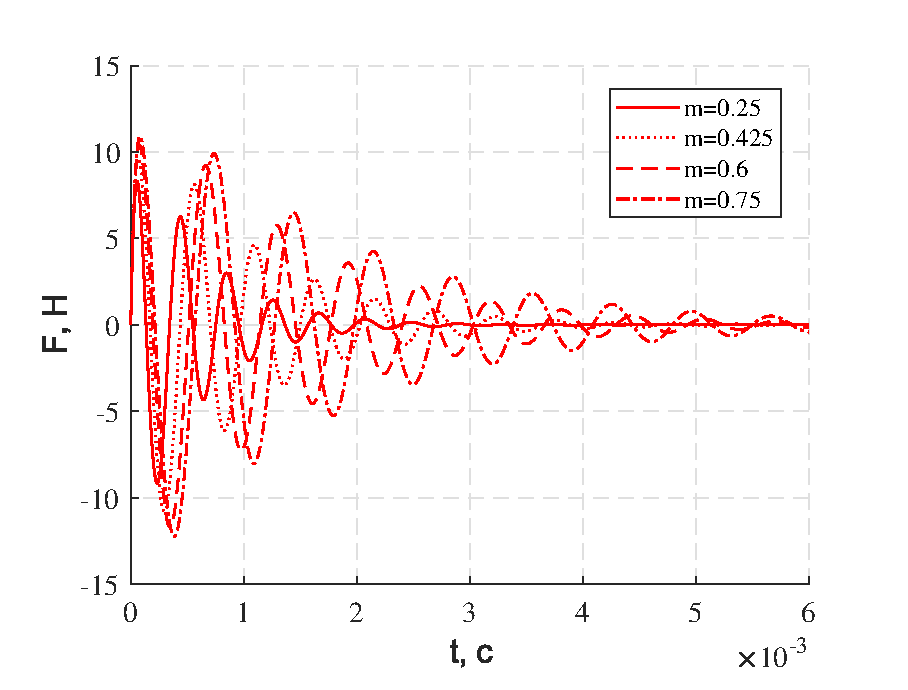
\includegraphics[width=1\linewidth]{f_pri_m.eps}} a) \\
			\end{minipage}
			\hfill
			\begin{minipage}[h]{0.47\linewidth}
				\center{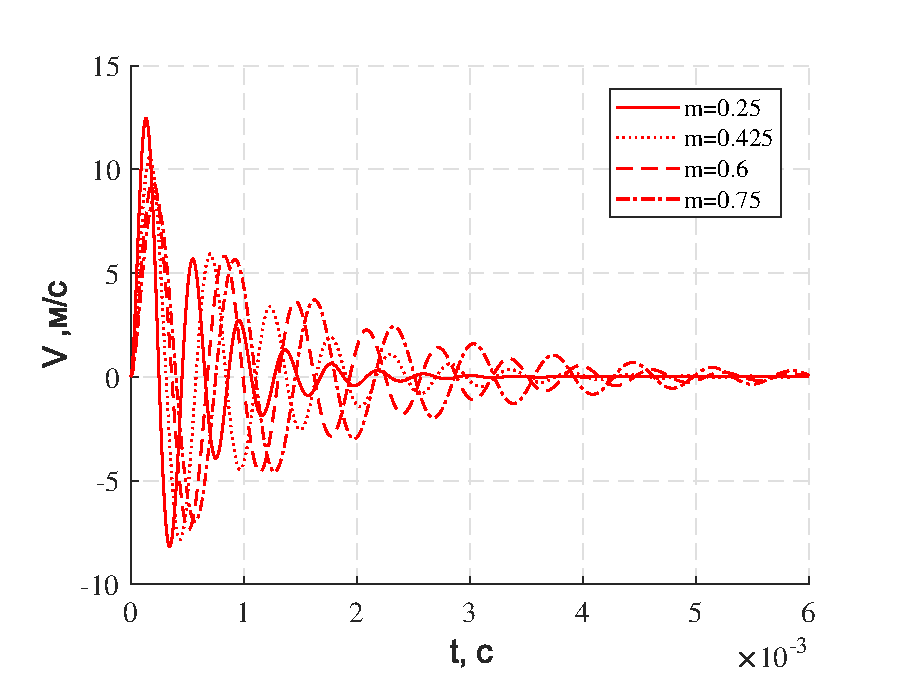
\includegraphics[width=1\linewidth]{v_pri_m.eps}} \\b)
			\end{minipage}
			\vfill
			\begin{minipage}[h]{0.47\linewidth}
				\center{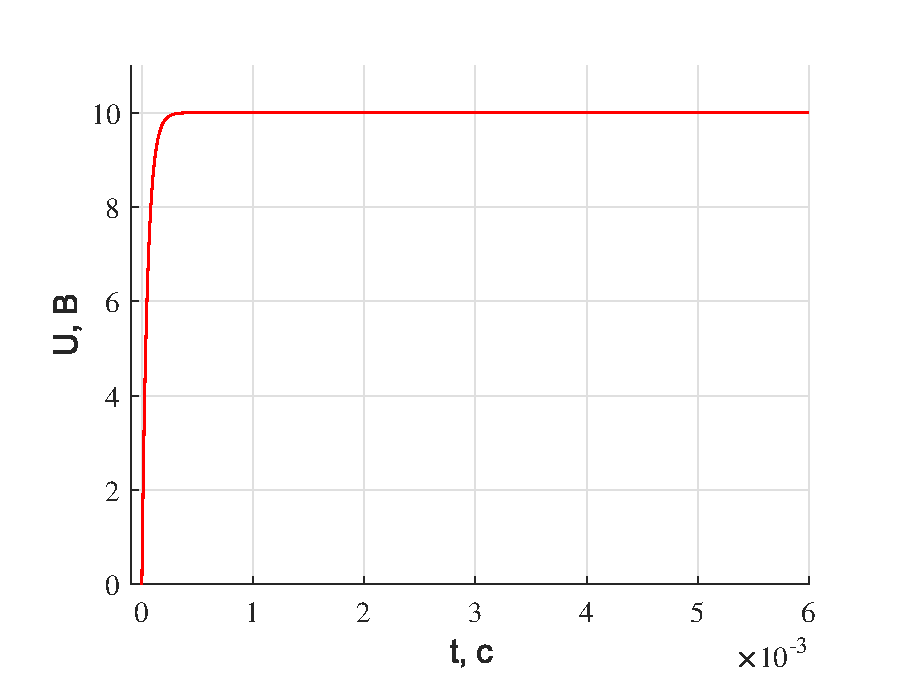
\includegraphics[width=1\linewidth]{um.eps}} c) \\
			\end{minipage}
			\hfill
			\begin{minipage}[h]{0.47\linewidth}
				\center{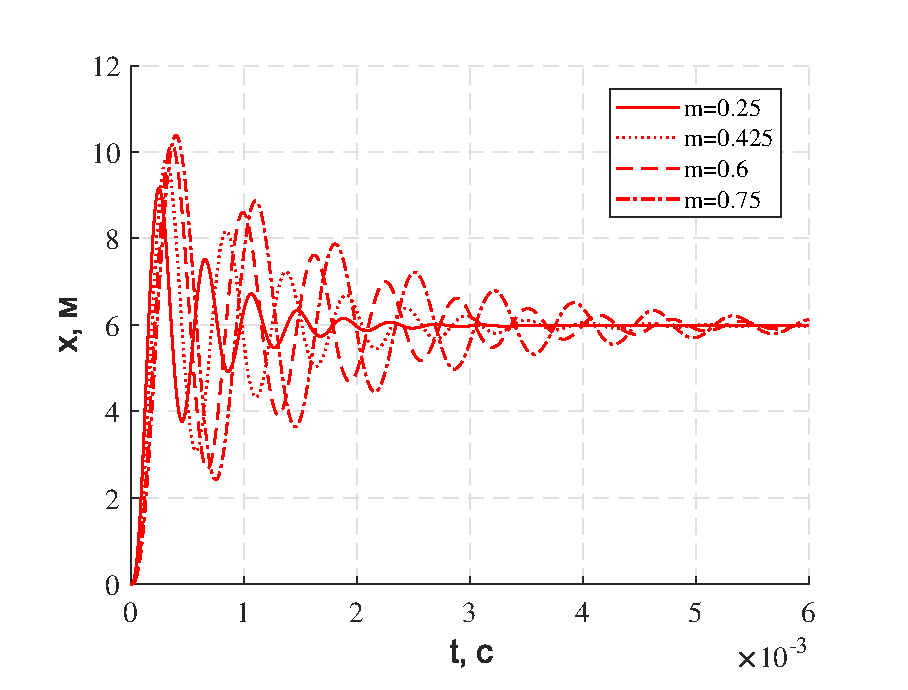
\includegraphics[width=1\linewidth]{x_pri_m.eps}} d) \\
			\end{minipage}
			\caption{Переходные процессы: a) динамическое усилие, b)
				скорость, c) напряжение, d) перемещение}
			\label{s_3}
		\end{figure}
	\newpage
	\paragraph{}Рассчитаем значения времени переходного процесса $t_\text{п}$, установившееся значение $x_y$ и перерегулирование $\sigma$ при различных $m$ для $x$. Результаты представлены в таблице \ref{t_2}
	\begin{table}[h]
		\centering
		\caption{Данные моделирования}
		\renewcommand{\arraystretch}{2} 
		\renewcommand{\tabcolsep}{1.6cm}
		\begin{center}
			\begin{tabular}{|c|c|c|c|}
				\hline
				$m$, кг & $t_\text{п} \cdot 10^4$,с & $x_y\cdot K_x$,м & $\sigma$(\%)  \\ \hline
				0.25 & 15 & 6 & 53 \\ \hline
				0.425 & 27 & 6 & 64 \\ \hline
				0.6 & 39 & 6 & 69 \\ \hline
				0.75 & 57 & 6 & 70 \\ \hline
				
			\end{tabular}
		\end{center}
		\label{t_2}
	\end{table}
	\newpage
	\begin{center}
	\section{Исследование влияния постоянной времени ВУ $T_u$ на вид переходных процессов}
	\end{center}
	
	\paragraph {} Графики переходных процессов при различных $T_u$ для каждого из исследуемых значений представлены на рисунке \ref{s_4}\\
	\begin{figure}[h!]
		\renewcommand{\figurename}{Рисунок}
		\begin{minipage}[h]{0.47\linewidth}
			\center{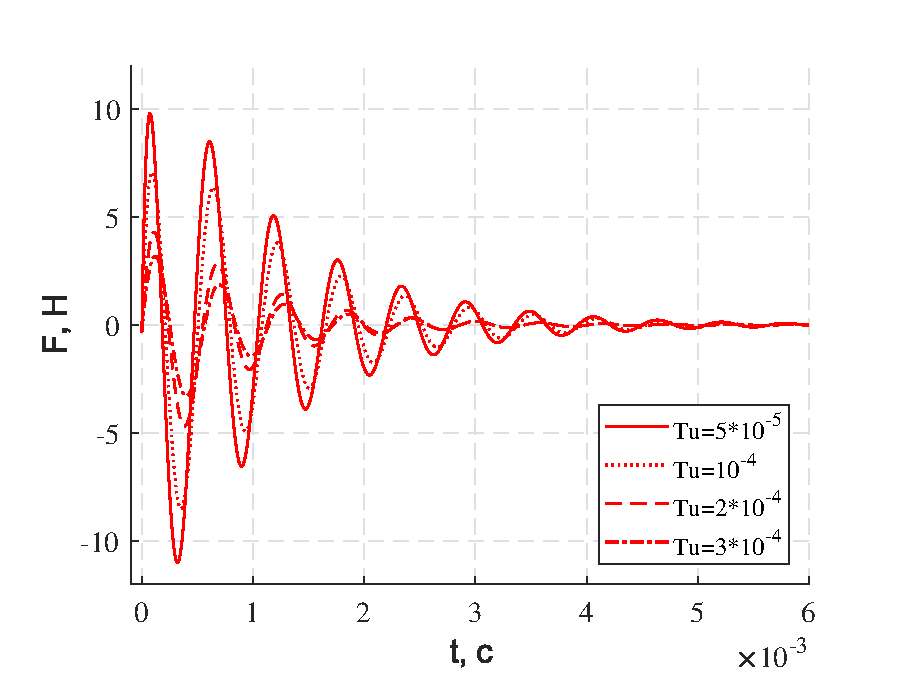
\includegraphics[width=1\linewidth]{ft.eps}} a) \\
		\end{minipage}
		\hfill
		\begin{minipage}[h]{0.47\linewidth}
			\center{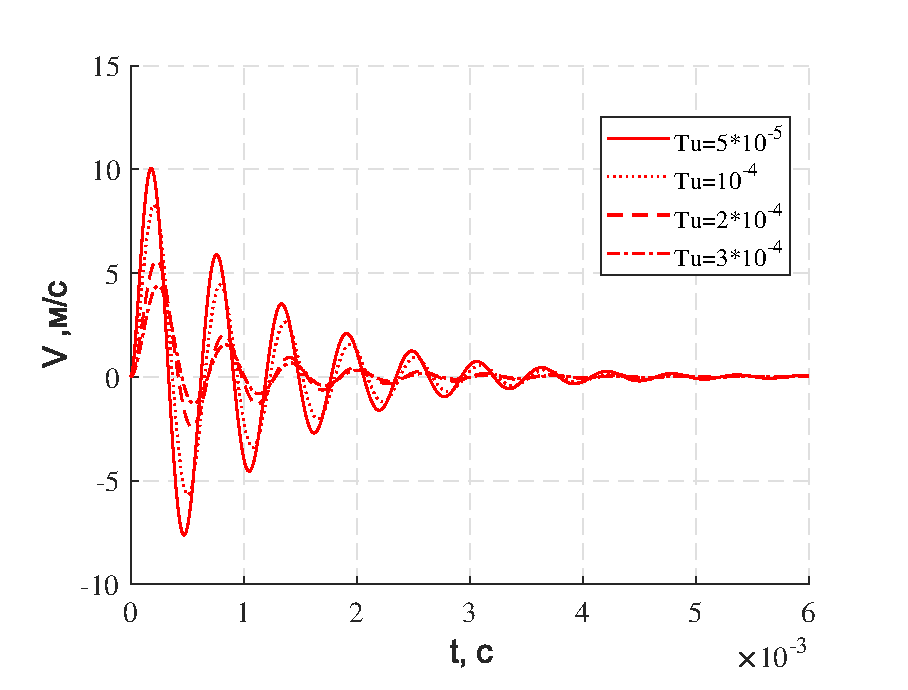
\includegraphics[width=1\linewidth]{v_pri_tu.eps}} \\b)
		\end{minipage}
		\vfill
		\begin{minipage}[h]{0.47\linewidth}
			\center{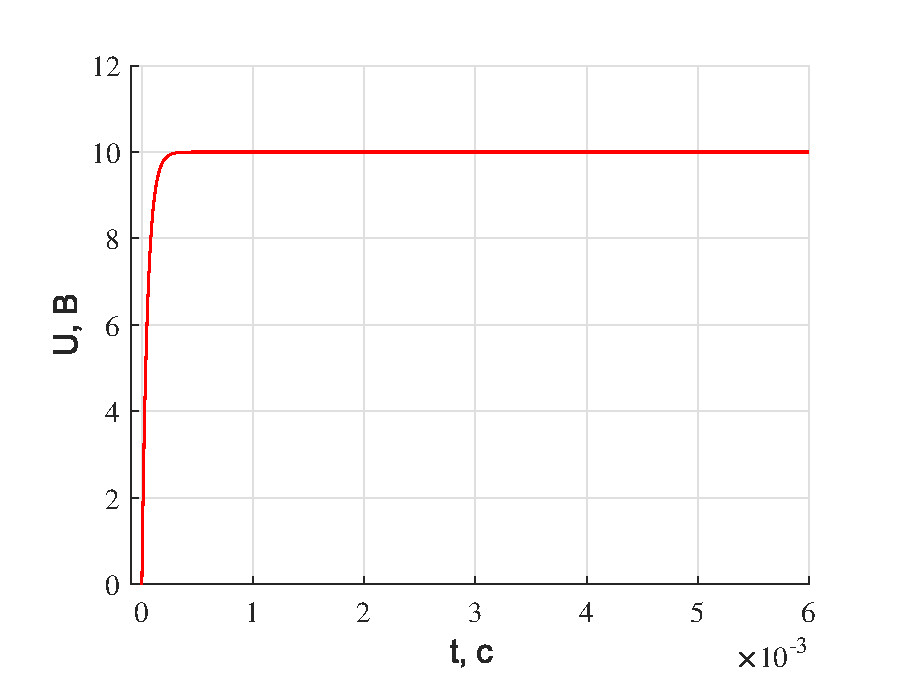
\includegraphics[width=1\linewidth]{ut.eps}} c) \\
		\end{minipage}
		\hfill
		\begin{minipage}[h]{0.47\linewidth}
			\center{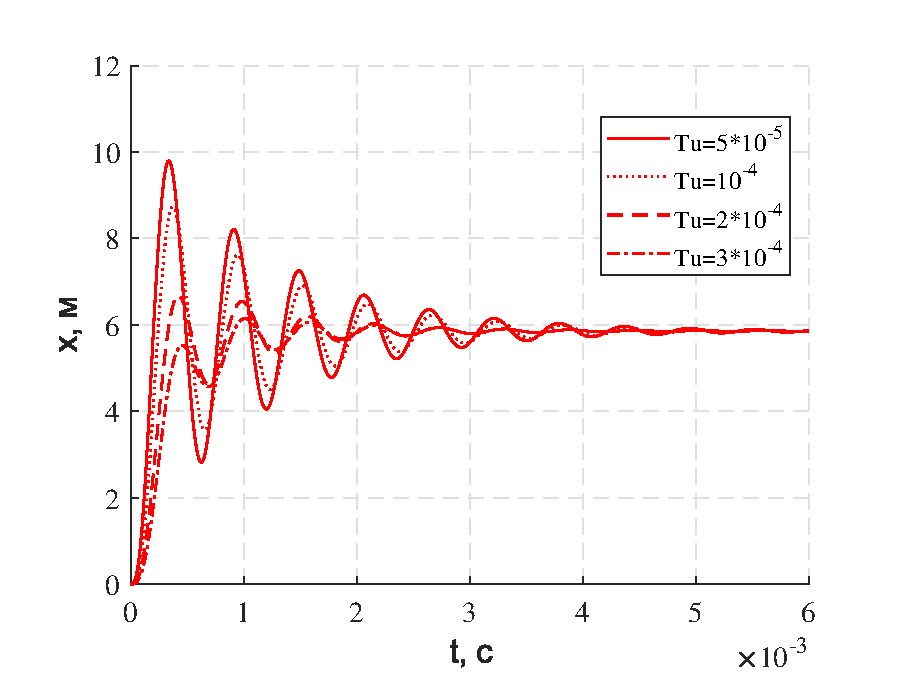
\includegraphics[width=1\linewidth]{xt.eps}} d) \\
		\end{minipage}
		\caption{Переходные процессы: a) динамическое усилие, b)
			скорость, c) напряжение, d) перемещение}
		\label{s_4}
	\end{figure}
	\newpage
	\paragraph{}Рассчитаем значения времени переходного процесса $t_\text{п}$, установившееся значение $x_y$ и перерегулирование $\sigma$ при различных $T_u$ для $x$. Результаты представлены в таблице \ref{t_3}
	\begin{table}[h]
		\centering
		\caption{Данные моделирования}
		\renewcommand{\arraystretch}{2} 
		\renewcommand{\tabcolsep}{1.45cm}
		\begin{center}
			\begin{tabular}{|c|c|c|c|}
				\hline
				$T_u\cdot 10^{4}$,с & $t_\text{п} \cdot 10^4$,с & $x_y\cdot K_x$, м & $\sigma$(\%)  \\ \hline
				0.5 & 30 & 6 & 67 \\ \hline
				1 & 27 & 6 & 49 \\ \hline
				2 & 16 & 6 & 14 \\ \hline
				3 & 14 & 6 & 5 \\ \hline
			\end{tabular}
		\end{center}
		\label{t_3}
	\end{table}
	
	Корни характеристического уравнения (\ref{v}) при $m=0.5,~C_p=0.6\cdot 10^8,~K_d=900$ и различных $T_u$:\\
	\begin{gather}
	(T_u s+1)(ms^2+K_d+C_p)=0 \label{v}
	\end{gather}
	\\
	
	\begin{itemize}
		\item При $T_u=0.5\cdot 10^{-4}: s_1=-2\cdot 10^4;~ s_{2,3}=-900\pm 10917.42i$\\
		\item При $T_u=1\cdot 10^{-4}~: s_1=-10^4;~ s_{2,3}=-900\pm 10917.42i$\\
		\item При $T_u=2\cdot 10^{-4}~: s_1=-0.5\cdot 10^4;~ s_{2,3}=-900\pm 10917.42i$\\
		\item При $T_u=3\cdot 10^{-4}~: s_1=-0.33\cdot 10^4;~ s_{2,3}=-900\pm 10917.42i$\\
	\end{itemize}
	
	
	\newpage
	\begin{center}
	\section{Исследование переходных процессов по возмущению}
	\end{center}
			\paragraph {} Графики переходных процессов $V$ и $x$ при $F_{\text{в}}$ и $U=0$ для различных значений коэффициента упругости $C_p$ представлены на рисунках \ref{s_5} и \ref{s_6} соответственно\\
			
			\begin{figure}[h!]
				\begin{center}
					\begin{minipage}[h]{0.45\linewidth}
						\renewcommand{\figurename}{Рисунок}
						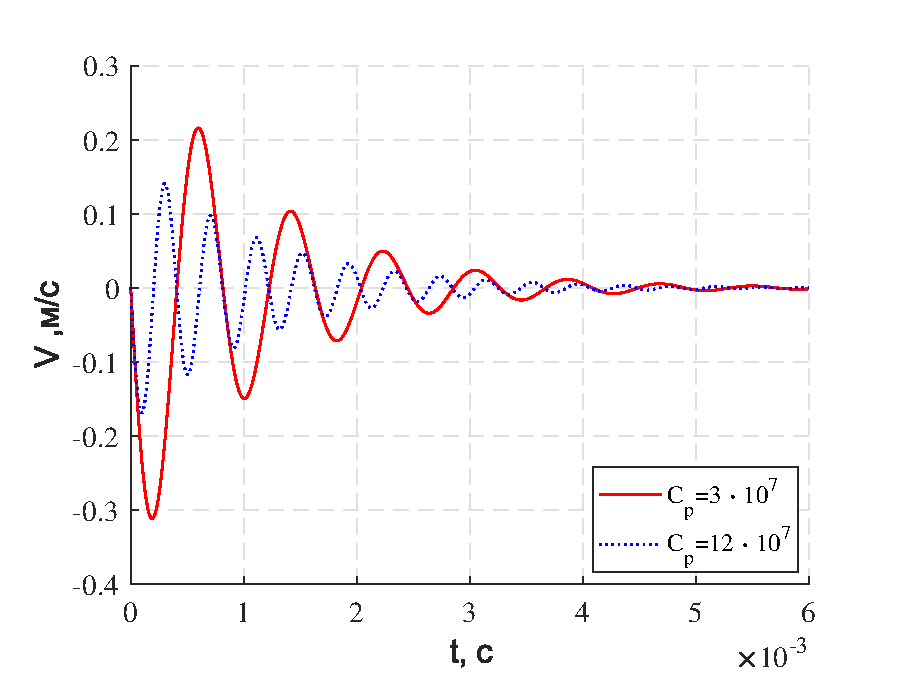
\includegraphics[width=1\linewidth]{v_pri_cp.eps}
						\caption{Переходные процессы для $V$} 
						\label{s_5} 
					\end{minipage}
					\hfill 
					\begin{minipage}[h]{0.45\linewidth}
						\renewcommand{\figurename}{Рисунок}
						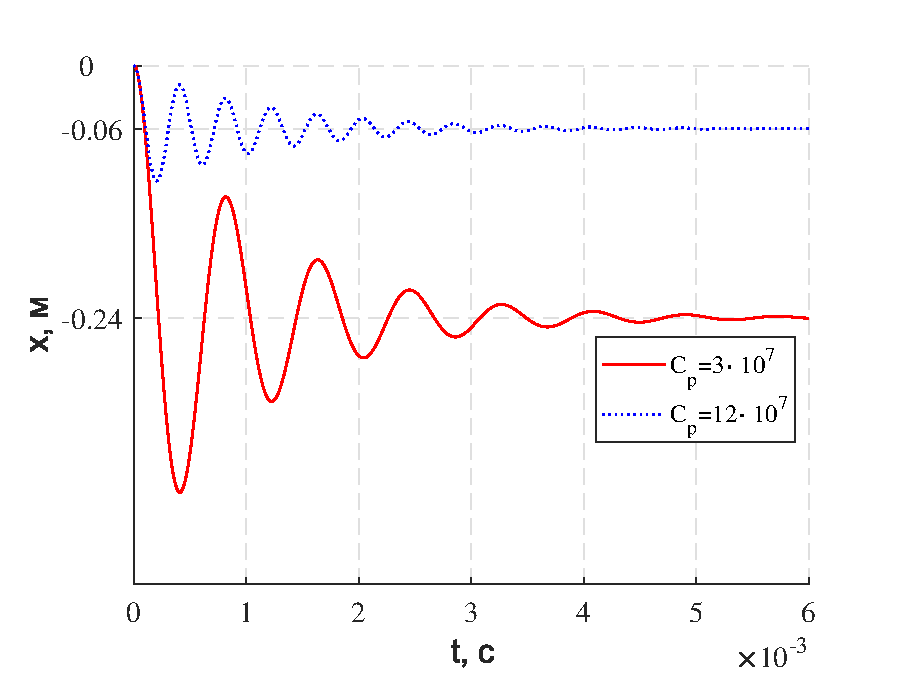
\includegraphics[width=1\linewidth]{x_pri_cp.eps}
						\caption{Переходные процессы для $x$}
						\label{s_6}
					\end{minipage}
				\end{center}
			\end{figure}	
	\newpage
	\begin{center}
		\section{Асимптотическая ЛАЧХ исполнительного устройтсва}
	\end{center}
	\paragraph{}
	Передаточная функция системы имеет вид, как было показано в 1 разделе(см. (\ref{v_3})):
	\begin{equation*}
	 W(s)=\frac{K_u\cdot K_o}{(T_u s+1)(ms^2+K_d s+C_p)}
	\end{equation*}
	Чтобы получить модуль частотной характеристики нужно взять отношение модулей числителя и знаменателя. В последнем в качестве второго множителя для приближенного анализа можно оставить только $C_p$. В итоге:
	\begin{gather}
	\displaystyle
	A(w)=\frac{K_u\cdot K_o}{C_p\cdot \sqrt{T_u^2 w^2+1}}
	\end{gather}	
	Асимптотическая ЛАЧХ представлена на рисунке \ref{s_7}
	\begin{figure}[h!]
			
		\centering
		\begin{tikzpicture}
		\begin{semilogxaxis} [
		width = 0.9\textwidth,
		ylabel = {$L(w)$, дБ},
		xlabel = {$w$, рад/c},
		xmin=1e3, xmax=1e6,
		extra x ticks = {2e4},
		extra x tick labels = {$\omega_c$},
		]
		\addplot [blue, mark=none, thick, solid] table [x={w}, y={L}] {data/laqc.dat};
		
		\draw [thick, dashed, black] (2e4, -145) -- (2e4,-105);
		\end{semilogxaxis}
		
		\end{tikzpicture}
		
		\caption{ЛАЧХ исполнительного устройства}
			\label{s_7}
	\end{figure}
	\\
	Сопрягающая частота $\displaystyle \omega_c=\frac{1}{T_u}=2\cdot10^4$
		\newpage
	\begin{center}
		\section*{Вывод} 
	\end{center}
	\par
	В данной работе была исследована математическая модель пьезоэлектрического исполнительного устройства. Были исследованы переходные характеристики некоторых величин и их зависимость от параметров системы.
	\par
	Было выявлено, что при увеличении массы нагрузки перерегулирование и время переходного процесса перемещения $x$ механизма. А при увеличении постоянной времени $T_u$ - наоборот. Установившееся значение остается неизменным.
	\par
	Также были найдены значения корней характеристического многочлена при различных значениях $Tu$, которые подтверждают характер переходного процесса - система устойчива (все 3 корня имеют отрицательную вещественную часть) и имеет склонность к колебаниям, так как есть пара комплексно-сопряженных корней.
	\par
	При возмущающем воздействии увеличение коэффициента упругости $C_p$ ведет к снижению амплитуды колебаний и уменьшению установившегося значения $x$. 
	
\end{document}